\subsubsection{Encoder Mode mit Hardware Timer}
\label{sec:Conf_Encoder}

Einige integrierte Timer im STM32 unterstützen einen Encoder Modus, bei dem 2 vorgegebene GPIO
Pins den Zählstand des Timers verändern können.
In der Konfiguration wird die Zählrichtung mit Counter Mode auf \texttt{Up} gesetzt.
Der maximale Zählerwert (Periode) ist der Maximalwert eines \texttt{uint16\_t} Datentyps $P_{max}=2^{16}-1=65's535$.
In Abbildung \ref{pic:CubeMX_TIM3} ist die Konfiguration für den Timer 3 dargestellt. Der Timer 4 erhält die selbe Konfiguration.

\begin{figure}[H]
	\centering
	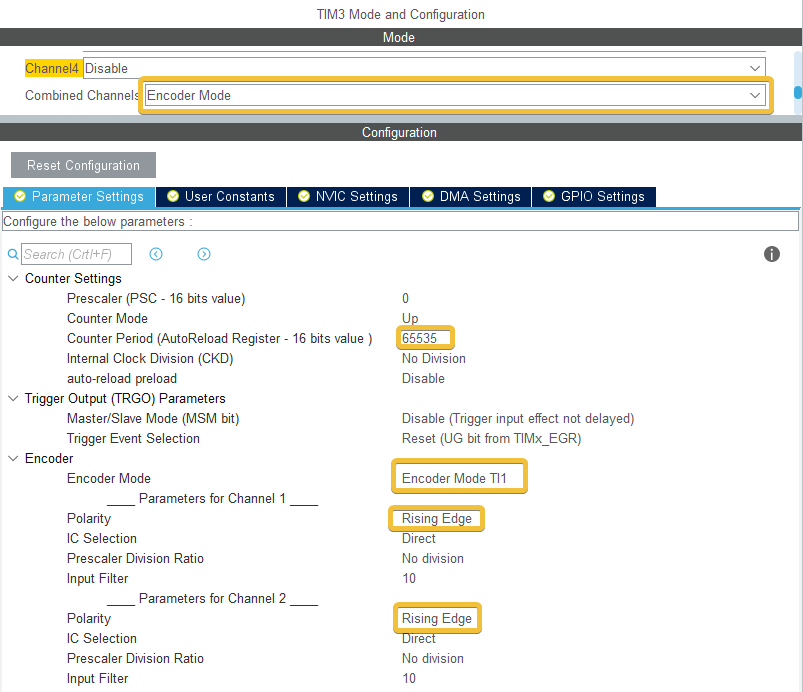
\includegraphics[width=0.9\linewidth]{CubeMX_TIM3}
	\caption{Konfiguration des Timer 3 im Encoder Modus}
	\label{pic:CubeMX_TIM3}
\end{figure}

\paragraph{Parameter}

Die nachfolgende Tabelle listet einige wichtige Parameter und deren Einfluss.

\begin{table}[H]
	\begin{tabular}{|l|l|l|}
		\hline
		\textbf{Setting} & \textbf{Werte} & \textbf{Erklärung}                            \\ \hline
		Counter Mode     & Up | Down      & Zählrichtung in Abhängigkeit der Drehrichung  \\ \hline
		Counter Period   &                & maximaler Zählerwert (z.b. uint16\_t)         \\ \hline
		Encoder Mode     & T1 | T2        & \begin{tabular}[c]{@{}l@{}}Triggerfokus auf CH1 oder CH2 oder beides.
			\\ Wenn beide aktiviert sind, zählt der Timer doppelt.\end{tabular} \\ \hline
	\end{tabular}
\end{table}

\paragraph{Anwendung im Code}

Das untenstehende Listing stellt dar, wie der Timer im \texttt{main.c} gestartet werden muss.
Eine Initialisierung alleine reicht nicht aus.

\begin{lstlisting}[language=c]
/* USER CODE BEGIN 2 */
// start Encoder mode on one channel
HAL_TIM_Encoder_Start(&htim2, TIM_CHANNEL_1);
/* USER CODE END 2 */
\end{lstlisting}

Mit dem unten gezeigten Befehl lässt sich der aktuelle Zählstand des Timers resp. Encoders auslesen.

\begin{lstlisting}[language=c]
/* USER CODE BEGIN x */
int new_encoder_val = TIM2->CNT;   // read encoder count anywhere in the code 
/* USER CODE END x */
\end{lstlisting}




